\subsection*{Database} \label{sec:databaseDesign}
Systemet skal, som nævnt i kravsspecifikationer, have forbindelse til en database. Denne kan tilgås fra den tilhørende controller. Klasserne for databasen og controlleren fremgår af \autoref{fig:MVCDatabase}. 

\begin{figure} [H]
\centering
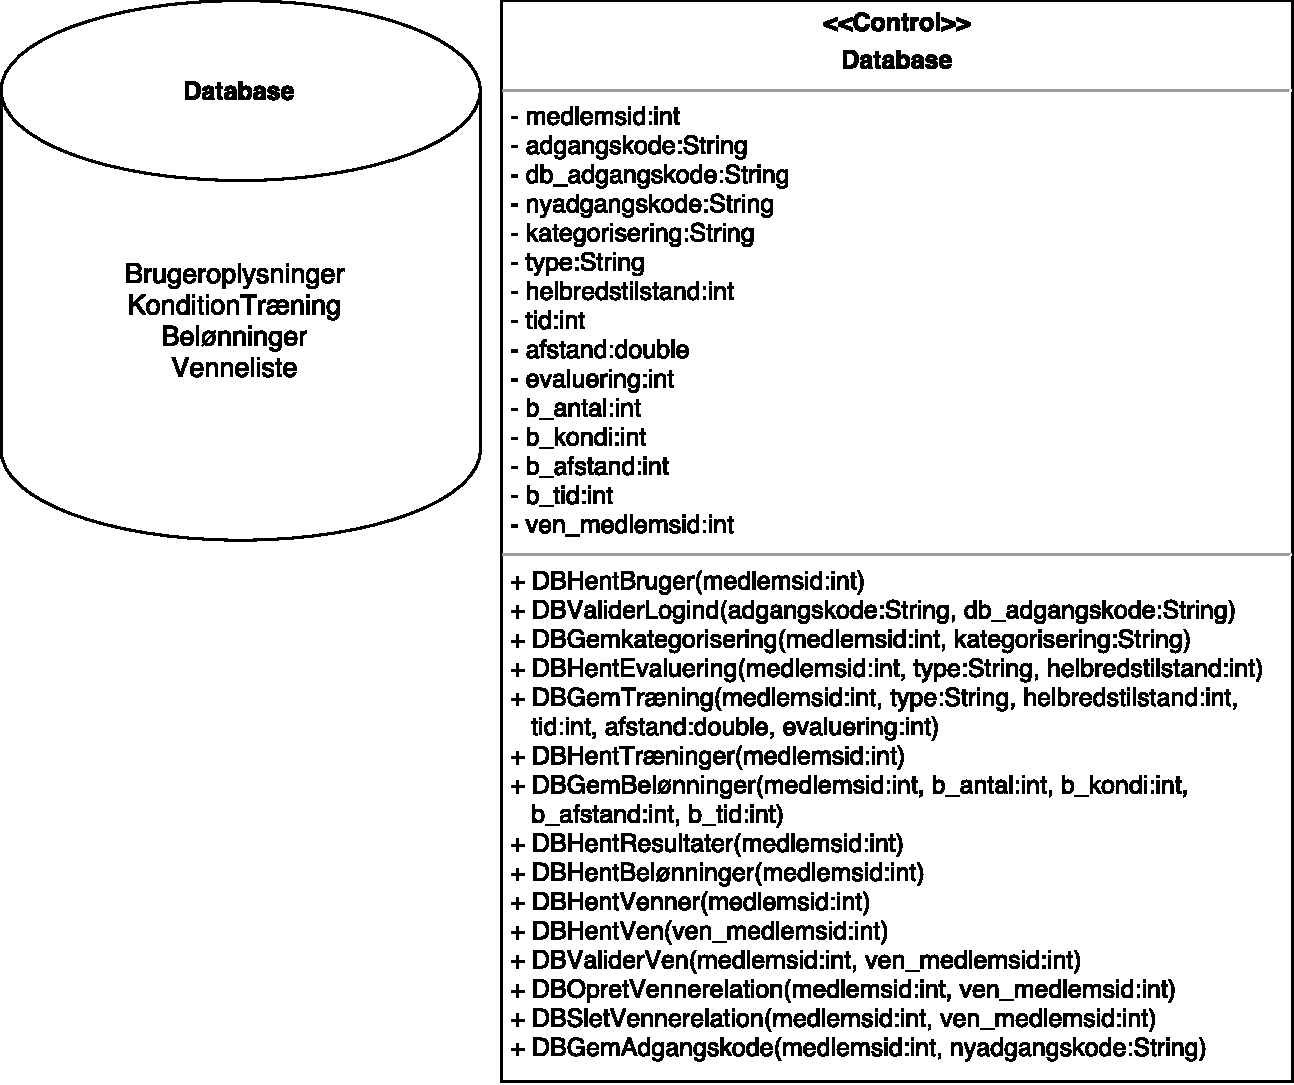
\includegraphics[width=0.7\textwidth]{figures/MVC/MVCDatabase}
\caption{Designklasse for Database. Til venstre ses databasen og til højre ses den tilhørende controller.}
\label{fig:MVCDatabase}
\end{figure}

\noindent
Databasen indeholder de oprettede tabeller Brugeroplysninger, KonditionTræning, Belønninger og Venneliste. Brugeroplysninger indeholder brugerens oplysninger, herunder medlemsID, navn og kategorisering. KonditionTræning indeholder brugerens resultater for de udførte konditionstræninger. Tabellen Belønninger lagrer værdier for de opnåede virtuelle belønninger. Vennelisten indeholder andre brugere som brugeren følger, derudover har brugeren mulighed for at tilføje eller fjerne brugere fra sin venneliste. Designet af databasen og tilhørende tabeller er yderligere beskrevet i et ER-diagram, der fremgår af \autoref{sec:ER}. 

\textit{Database} controlleren indeholder attributter og metoder. De tilhørende attributter og metoder er private, da det ikke ønskes at ændre eller tilgå disse fra andre controllere. Dertil skaber det en større kontrol samt mindsker fejl i forhold til uhensigtsmæssige ændringer. Attributtens type vil fremgå efter den tilhørende attribut. Metoderne for dennne controller er henholdsvis Hent, Valider, Gem, Opret og Slet. Disse metoder udføres i forhold til definerede inputsparametre, hvilket er angivet i parenteser.

Metoderne har til formål at kommunikere mellem databasen og de forskellige controllere. Der oprettes forbindelse til databasen ved samtlige controllere. 

\subsection*{Lagring af data}  \label{sec:entity}
Når der oprettes forbindelse til databasen i forbindelse med, at brugeren logger ind eller tilgår resultater på app'en, sendes og gemmes data i forskellige entitys, som fremgår af \autoref{fig:MVCEntity}. Der er valgt at udarbejde entitys for at lagre data midlertidig førend det sendes til databasen. 

\begin{figure} [H]
\centering
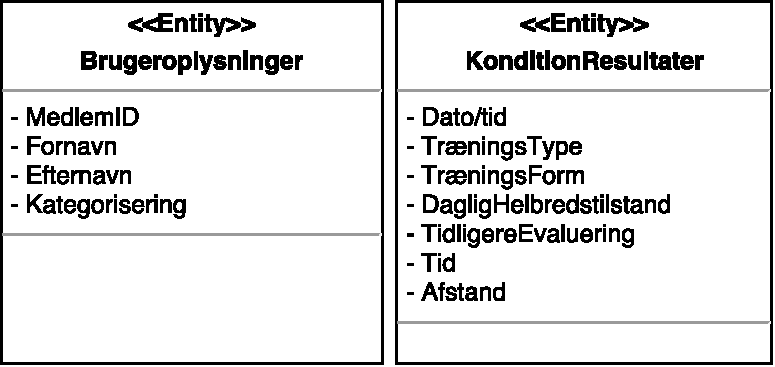
\includegraphics[width=0.5\textwidth]{figures/MVC/Entity}
\caption{Designklasser for entitys, herunder Brugeroplysninger og KonditionResultater. Attributterne er markeret med \-, hvilket indikerer, at disse er privat.}
\label{fig:MVCEntity}
\end{figure}

\noindent
På \autoref{fig:MVCEntity} fremgår det, at de forskellige attributter er private. Dette er gjort, da det ønskes, at attributterne kun kan tilgås indenfor det samme klasse. 
\textit{Brugeroplysninger} indeholder informationer om brugeren, herunder MedlemsID, Fornavn, Efternavn og Kategorisering. 
\textit{KonditionResultater} indeholder brugerens resultater, som er defineret ud fra DatoTid, TræningsType, TræningsForm, DagligHelbredstilstand, Evaluering, Tid og Afstand. 
